\chapter{Controleren op kwaliteitsgebreken}\label{sec:kwaliteitsgebrek}
In dit hoofdstuk beschrijven we een alternatieve voorstellingsmethode voor klassediagrammen waarmee we bepaalde soorten kwaliteitsgebreken kunnen detecteren. Waar in hoofdstuk \ref{sec:consistentie} objecten centraal stonden, doen we daar hier afstand van: We abstraheren de logische types voor klasses weg en concentreren ons in de plaats op \textit{ClassObject}, een logisch type dat een overeenkomstig object heeft voor alle klasses in het diagram. We gebruiken het diagram in figuur \ref{fig:diagram-voorbeeld} weer als begeleidend voorbeeld. In de volgende subsecties overlopen we hoe we de theorie die we gebruiken voor dit probleem opbouwen.

\section{Gebruikte logische types en predicaten}
\sloppy Waar we in sectie \ref{sec:hierarchies} het logisch type \textit{ClassObject} en het predicaat \\ \textit{IsSupertypeOf/2} afwezen, behouden we ze hier en berekenen we de transitieve sluiting van \textit{IsSupertypeOf/2} zoals beschreven in diezelfde sectie.

We gebruiken daar bijkomend de volgende nieuwe logische symbolen:

\begin{itemize}
	\item \textbf{\textit{BiAssoc(ClassObject,ClassObject)}}: drukt uit dat er een binaire associatie bestaat tussen de twee klasses.
	\item \sloppy \textbf{\textit{BiAssocLow(ClassObject,ClassObject,ClassObject) : nat}}: voor \\ \textit{BiAssocLow(x,y,x) = n1} geldt dat voor de binaire associatie tussen klasse \textit{x} en klasse \textit{y} de ondergrens voor de multipliciteit aan de \textit{x}-kant gelijk is aan \textit{n1}; een gelijkaardige interpretatie geldt voor \textit{BiAssocLow(x,y,y) = n2}.
	\item \textbf{\textit{BiAssocHigh(ClassObject,ClassObject,ClassObject) : nat}}: gelijkaardig aan \textit{BiAssocLow/3}, maar dan voor de bovengrens van de multipliciteit.
\end{itemize}

Deze predicaten worden ingevuld met een lijst van feiten die af te lezen zijn van het diagram.

\section{Kwaliteitsgebreken detecteren}
Er zijn drie kwaliteitsgebreken waarnaar wordt gezocht in de resulterende theorie:

\begin{itemize}
	\item \textbf{\textit{Many-to-many} associaties}: Dit zijn associaties waar de bovengrens van de multipliciteiten aan beide kanten gelijk is aan $*$. Het voorkomen van een \textit{many-to-many} associatie is doorgaans een teken dat er een klasse ontbreekt in het ontwerp. Het is dus van groot belang dat dit wordt opgespoord en opgelost.
	
	\item \textbf{Losstaande klasse}: Concreet is een losstaande klasse een klasse die geen associatie heeft met een andere klasse in het ontwerp. Zulk een klasse is nutteloos en moet ofwel verbonden worden met een andere klasse of verwijderd worden.
	
	\item \textbf{Overbodige associaties in een klassehi\"erarchie}\cite{Balaban2015}: Beschouw figuur \ref{fig:hierarchie}. De associatie \textit{Alice}---\textit{Bob} heeft tot gevolg dat er exact even veel instanties van \textit{Alice} zijn als instanties van \textit{Bob}. De associatie \textit{Charlie}---\textit{David} stelt echter dat elke instantie van \textit{David} in verband staat met hoogstens vijf instanties van \textit{Charlie}. In een correct model voor dit diagram staat elke instantie van \textit{David} in verband met exact \'e\'en instantie van \textit{Charlie}. De bovengrens van vijf op het uiteinde \textit{Charlie} is dus niet precies genoeg en zou moeten gelijkgesteld worden aan \'e\'en om de verstaanbaarheid van het diagram te verbeteren.
\end{itemize}

We defini\"eren deze respectievelijke gebreken in de logische theorie door middel van de volgende logische zinnen:

\begin{align}
	\nonumber \forall{x}[ClassObject]\forall{y}[ClassObject](ManyToMany(x,y) \Leftrightarrow BiAssoc(x,y) \land \\ \lnot\exists{z}[nat](BiAssocHigh(x,y,x) = z) \land \lnot\exists{z}[nat](BiAssocHigh(x,y,y) = z)).\label{form:manytomany}
\end{align}

\begin{align}
	\nonumber \forall{x}[ClassObject](LooseClass(x) \Leftrightarrow \lnot(\exists{y}[ClassObject](\lnot(x = y) \land (BiAssoc(x,y) \\ \lor \exists{s}[ClassObject]\exists{y}[ClassObject](\mathit{IsSupertypeOf}(s,x) \land BiAssoc(s,y)))))).\label{form:loose}
\end{align}

\begin{align}
	&\nonumber\forall{x}[ClassObject]\forall{y}[ClassObject](SubclassImpreciseUpperBound(x, y, x) \Leftrightarrow \\
	&\nonumber\exists{sx}[ClassObject]\exists{sy}[ClassObject]
	(((sx = x \land IsSupertypeOf(sy, y)) \lor \\
	&\nonumber(IsSupertypeOf(sx, x) \land sy = y) \lor \\
	&\nonumber(IsSupertypeOf(sx, x) \land IsSupertypeOf(sx, y))) \\
	&\nonumber\land BiAssoc(x, y) \\
	&\nonumber\land BiAssoc(sx, sy) \\
	&\nonumber\land BiAssocLow(sx, sy, sx) = BiAssocLow(sx, sy, sy) = BiAssocHigh(sx, sy, sx) = \\
	&\nonumber{}BiAssocHigh(sx, sy, sy) \\ 
	&\land BiAssocHigh(x, y, x) > BiAssocLow(sx, sy, sx))\label{form:imprecise-bound}.
\end{align}

\begin{figure}
	\centering
	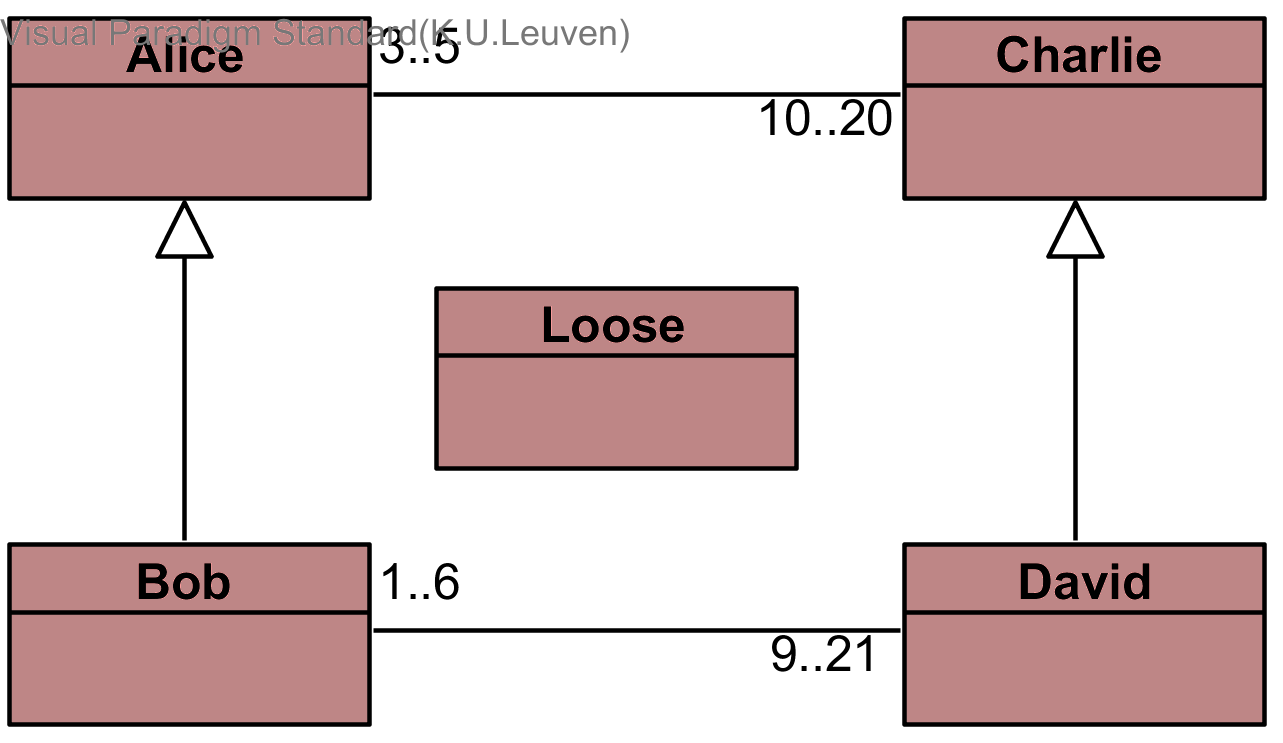
\includegraphics{chap-kwaliteitsgebrek/hierarchy.png}
	\caption{Voorbeeld van een onvoldoende precieze bovengrens in een klassehi\"erarchie en van een losstaande klasse (zijnde \textit{Loose})}
	\label{fig:hierarchie}
\end{figure}

Zin \ref{form:manytomany} controleert of voor beide rollen van een associatie geldt dat de bovengrens * is.

Zin \ref{form:loose} controleert of klasse \textit{x} rechtstreeks geassocieerd is met een andere klasse, en zoniet, of klasse \textit{x} een subklasse is van een andere klasse en of die superklasse geassocieerd is met nog een andere klasse.

Zin \ref{form:imprecise-bound} controleert op patronen van klassehi\"erarchie\"en en associaties zoals in diagram \ref{fig:hierarchie}. Daarbij worden gevallen waar het equivalent van \textit{Alice} ontbreekt en gevallen waar het equivalent van \textit{Bob} ontbreekt ook opgespoord. De zin controleert of er een associatie bestaat tussen de subklasses en of er een associatie bestaat tussen de superklasses. Zo ja, dan wordt de bovengrens op een uiteinde in een associatie tussen de subklasses aangeduid als onvoldoende precies indien:

\begin{itemize}
	\item Beide uiteindes van de associatie tussen de superklasses hebben een multipliciteit van de vorm $n..n$.
	\item De bovengrens op het uiteinde in een associatie tussen de subklasses is groter dan $n$.
\end{itemize}

Bijlage \ref{app:kwaliteitsgebrek} bevat de theorie die werd gegenereerd uit een combinatie van diagrammen \ref{fig:diagram-voorbeeld} en \ref{fig:hierarchie}. IDP
vindt alle \textit{many-to-many} associaties, besluit dat \textit{Loose} een losstaande klasse is en dat de bovengrens op \textit{Charlie} in de associatie \textit{Charlie}---\textit{David} onvoldoende precies is.